\chapter{Theoretische Grundlagen}
\label{chap:two}
\section{Bibliothek und Statistik}
\label{chap:two_one}
Bibliotheksrahmen - Etatplanung - Etatbedarfe, Zielsetzung der Bibliothek\\
Begriffe wie Mittelallokation\\
Bestandsmanagement\\
Was ist Statistik\\
Erhebung von qualitativen und quantitativen Daten Bsp.:\\
Konzentration auf quantitative Daten wie ...\\
hat schon immer große Rolle in Bibliotheken gespielt\\
BIX, Deutsche Bibliotheksstatistik (seit wann)\\
Warum ist Messbarkeit von bibliothekarischen Daten wichtig?\\
Welchen Impact für Budgetplanung können statistische Daten haben?\\
Was können statistische Daten in Bibliotheken aussagen?\\
Welche Daten werden in Bibliotheken erhoben\\
Sammlungsbezogene Evaluierung
Nutzerbezogene Evaluation\\
Nutzungsbezogene Evaluation\\
quantitativ und qualitativ:\\
Counter-Statistiken \& Standards\\

\clearpage

\section{Datenvisualisierung}
Mit den Siegeszug des Computers in den 1980/90er Jahren sind \dots\\
Was ist unter Datenvisualisierung zu verstehen?\\
leicht verschiedene Begriffsdefinitionen
Vielzahl von Begriffen\\ 
Oberbegriff für Informationsvisualisierung / Scientific Visualization\\
Abgrenzung zu Infographics\\
Zu welchem Zweck\\
Eigenschaften\\
Wie Datenvisualisierungen gestaltet werden sollen - simpel\\
Grundlage - Daten - quantitativ / qualitativ
Warum Datenvisualisierung wichtig ist?\\
Was erzählen Datenvisualisierungen mehr als Zahlenkolonnen?\\
Perception of the eye - schnellere Auffassung
Welche Datenvisualisierungen gibt es?\\
Wo kommen Daternvisualisierungen zum Einsatz?\\



% \begin{figure}[ht]
%     \centering
%         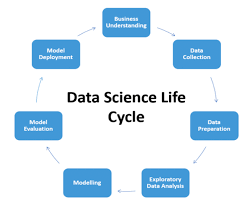
\includegraphics[width=8cm]{ds_cycle}
%         \caption{Data Science Cycle}
%         \label{fig:data science}
% \end{figure}



\clearpage
\section{Business-Intelligence-Systeme}

Was sind Business-Intelligence-Löungen?\\
Wo kommen Buisiness-Intelligence-Lösungen zum Einsatz zum Einsatz?
